\chapter{Experiments}

This chapter introduces the line of experiments taken out in this work and their intermediate conclusions. Initially, basic experiments about the detection of \acp{EWFO} are conducted. In further steps the insights are applied when transferring to the more challenging environment of autonomous drone races. Finally, a detector for \acp{EWFO} is deployed on an example \ac{MAV}.

\section{Experimental Setup}

The section gives a general description of the training and evaluation process. The hardware and software used to train the models are explained. Furthermore a description of particular plots used for evaluation is given.

\subsection{Training}

\textit{YoloV3} is differentiable and can thus be trained with gradient descent. However, with large amounts of data and high amount of parameters this algorithm has a slow update rate. Hence, \textit{Adam}\cite{Kingma2014}, a version of stochastic gradient descent is used. Thereby the gradient is estimated based on a subsample of the training set. While this leads to faster convergence, estimation errors can cause updates in the wrong direction. \textit{Adam} compensates for this by not only taking the mean gradient into account but also its first and second statistical moment. The three moments are weighted with $\alpha$,$\beta_1$ and $\beta_2$, where $\alpha$ is also referred to as learning rate. This work uses the parameters recommended in the initial public publication of \textit{Adam}\cite{Kingma2014}:

$$\alpha=0.001 \quad \beta_1=0.9 \quad \beta_2=0.999$$

An optimization process such as the training of a \acp{CNN} depends on the initialization of its parameters. \citeauthor{Glorot2010} \cite{Glorot2010} propose to initialize weights based on a uniform distribution centered around zero, where the borders depend on the input size of the layer. This scheme is a standard in Deep Learning frameworks and also used in this work.

Similarly to the network architectures and loss functions, the training procedure is implemented with \textit{keras} and \textit{tensorflow}-backend. All trainings are carried out on a Nvidia Pascal GTX 1080 Ti GPU with 3584 cores and 11GB RAM.

Machine Learning based Object Detection aims to recognize objects on unseen samples. Hence, 0.1 \% of the training samples are used as validation set. The training is stopped when the validation error converges; that is when it does not decrease for more than $1e^{-08}$ in 3 epochs.

\subsection{Testing}

The detector is tested by inferring the network on a given test set and calculate the metrics described in \Cref{sec:metrics}. While this gives a good estimation about the overall performance of a network it can be required to investigate the results in greater detail. It can be important to now how the detector deals with certain view points for example. In order to perform this evaluation predictions and true labels are assigned on bins based on certain conditions e.g. the bounding box size. Subsequently the performance is evaluated only for each bin individually.

In special cases it can happen that a bin border falls right between a true and a predicted label. For example a prediction is of size 10 a predicted label of size 12 and the border is at size 11. Even if the detection is correct this separation would lead to counting a missing detection as well as a false positive in each of the bins. Hence, the performance for the individual bins is typically a bit lower than when calculating a metric for the whole dataset.

The training algorithm as well as the network initialization are random processes. Hence, the network weights after training, as well as its performance are not deterministic. This condition has to be taken into account when interpreting the results. Ideally, each training is performed repeatedly and mean and standard deviation are used for evaluation. However, the training of \acp{CNN} takes a considerable amount of time which is why not all experiments can be taken out with many repetitions. Instead, trainings are performed at least two times and only further repeated if the two results have a high deviation. In plots an error bar displays the standard deviation between the different repetitions.

\section{Studying emptiness}

\acp{CNN} combine simple local features to more complex patterns layer by layer. Thereby pooling removes task irrelevant information and reduces the spatial dimension. In the deeper layers features of larger areas in the image are combined and encoded in an increasing amount of filters. In the final layer each location in the volume encodes the patterns that are present in the respective field of the preceding filters and an object prediction is performed.

The power of deep \acp{CNN} arises from their capability to learn very complex patterns. However, these are not present in \acp{EWFO}. Instead most of the object area consists of background and should be ignored by the detector. We hypothesize that this emptiness makes the detection more difficult than the detection of other objects as the detector can not exploit complex patterns. Instead any object can be present within the frame and thus distract the detector.

The combination of emptiness and simple features can have further implications on the training of an Object Detector for \acp{EWFO}. If not sufficient variations in background is provided in the training set, a detector is likely to overfit to the background of the training set. This condition can be amplified for more complex architectures with more parameters.

To summarize our hypotheses are:
\begin{enumerate}
	\item Compared to a simple filled object, the detection of \acp{EWFO} is harder, as the object does not provide complex patterns and a detector can be objects that are present in the empty part. Hence, the performance will decrease for objects that are far away (as the features are thin and hardly visible) and the performance will decrease for close objects, when the empty part gets larger.
	\item Compared to a complex filled object, the detection of \acp{EWFO} can not be improved by using a deeper network.
	\item Compared to other objects \acp{EWFO} do depend more on background. If the environment in the training set is different to the test set, the performance drop for \acp{EWFO} is higher than for other objects. This performance drop is larger for a more complex network.
\end{enumerate}

In order to evaluate these hypotheses the detection of \acp{EWFO} is compared to the detection of filled objects. Two examples are chosen by augmenting the empty part of the object with a pattern. The patterns are visualized in \Cref{fig:cats}. Thereby a simple object is chosen such as the stop sign which is clearly distinguishable from the background. This is compared to a more complex object such as the cat image.

\begin{figure}[hbtp]
	\centering
	\begin{minipage}{0.3\textwidth}
		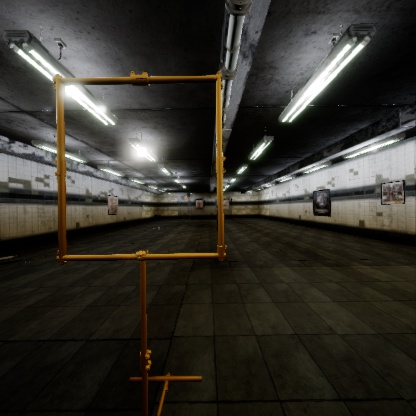
\includegraphics[width=\textwidth]{fig/gate}
	\end{minipage}
	\begin{minipage}{0.3\textwidth}
		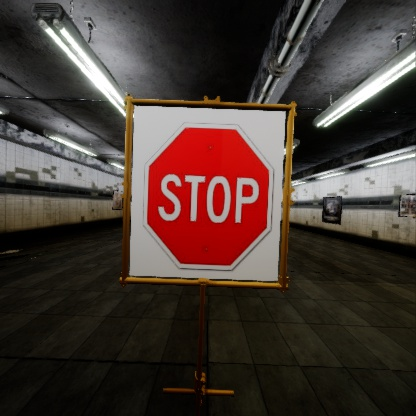
\includegraphics[width=\textwidth]{fig/sign}
	\end{minipage}
	\begin{minipage}{0.3\textwidth}
		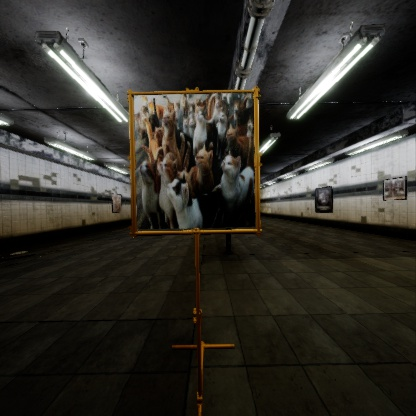
\includegraphics[width=\textwidth]{fig/cats}
	\end{minipage}
	\caption{Examples of the three objects that are compared. The \acp{EWFO} object left is compared to a simple solid object in the center and a complex solid object on the right.}
	\label{fig:cats}
\end{figure}

\subsection{Training Set}

For each object a dataset with 10 000 samples is created within the \textit{Basement} environment. As this experiment focuses on the influence of the empty part of the object, the view points are limited to frontally facing the object in various distances . On these training sets multiple architectures are trained: 

\begin{itemize}
	\item \textit{SmallYoloV3}
	\item \textit{VggYoloV3}
\end{itemize}


\subsection{Test Set}

For each object a test set of 150 samples is created within the \textit{Basement}-Environment, as well as the \textit{IROS}-Environment. Hence, in total there are 6 test sets with 150 samples each. Similar to the training set the view points are limited to frontally facing the object at various distances.


\subsection{Results}

\begin{table}
	\centering
	\input{tables/shallow_basement.txt}
    \caption{Performance in \ac{mAP} in the \textit{Basement} Environment. Each trained network (row) is evaluated on each test set (column). It can be seen how the detectors exploit the structure that is placed in the object. When it is removed the performance drops. Similarly, the performance drops when the detector for \ac{EWFO} sees a structure inside the object. }
\end{table}

\begin{table}r
	\centering
	\input{tables/shallow_iros.txt}
	\caption{}
	
\end{table}


\begin{figure}
	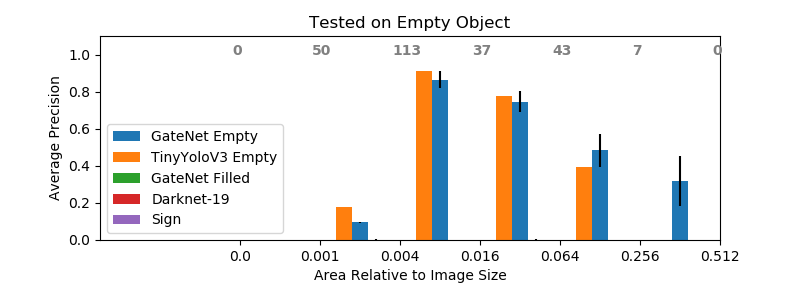
\includegraphics[width=\textwidth]{fig/basement_gate_size}
	\caption{An example of the augmented object. A \acp{CNN} can exploit this structure and should be less distracted by background.}
	\label{fig:basement_gate}
\end{figure}

\begin{figure}
	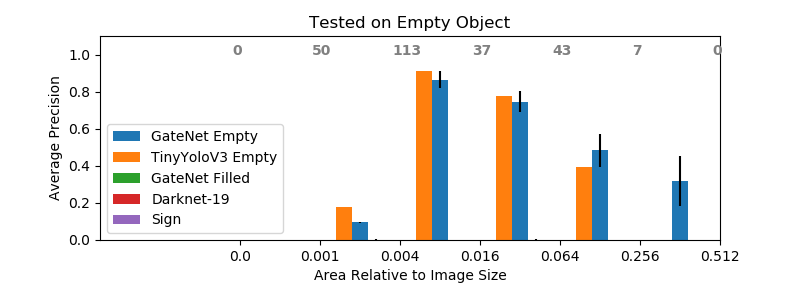
\includegraphics[width=\textwidth]{fig/basement_gate_size}
	\caption{An example of the augmented object. A \acp{CNN} can exploit this structure and should be less distracted by background.}
	\label{fig:basement_sign}
\end{figure}

\begin{figure}
	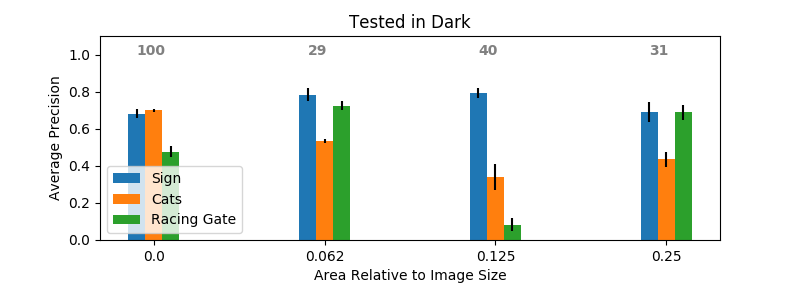
\includegraphics[width=\textwidth]{fig/basement_cats_size}
	\caption{An example of the augmented object. A \acp{CNN} can exploit this structure and should be less distracted by background.}
	\label{fig:basement_cats}
\end{figure}

\subsection{Discussion}

\subsection{Conclusion}

\section{Filling the hole}

The context in which an object is placed consists of background as well as light conditions or other objects. It is determined in the first step of the data generation process. Theoretically \acp{CNN} can learn to exploit context for detection. Yet, the actual influence is not clear. For example the Object Detectors trained in \cite{Peng} do not seem to make use of this image cue. Nevertheless, we investigate the importance of context for the detection of \acp{EWFO}. We hypothesize that due to the sparsity of their features and their emptiness context and background plays a more important role than for solid objects.

For the investigation we compare three methods to generate data: The placement of \ac{CAD}-models on uniformly coloured backgrounds, on backgrounds taken from a dataset as well as from fully synthesized environments. In terms of geometric and physical properties the fully synthesized environments provide the most realism and hence should give the best results. However, as the graphical engine only contains a limited set of textures, the variance in background is way smaller than in the backgrounds taken from a dataset. Furthermore, the objects in the background are also rendered. Hence, when tested on real data this method could lead to better performance.


\begin{figure}[hbtp]
	\centering
	\begin{minipage}{0.3\textwidth}
		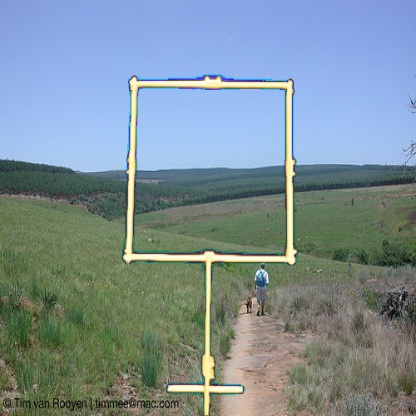
\includegraphics[width=\textwidth]{fig/voc}
	\end{minipage}
	\begin{minipage}{0.3\textwidth}
	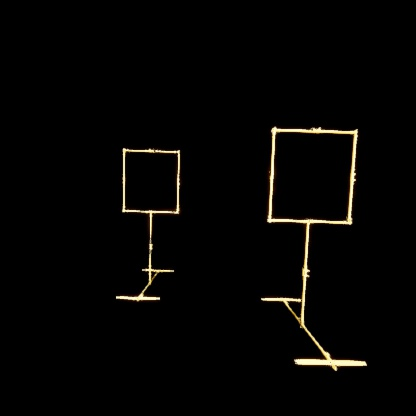
\includegraphics[width=\textwidth]{fig/void}
	\end{minipage}
	\begin{minipage}{0.3\textwidth}
		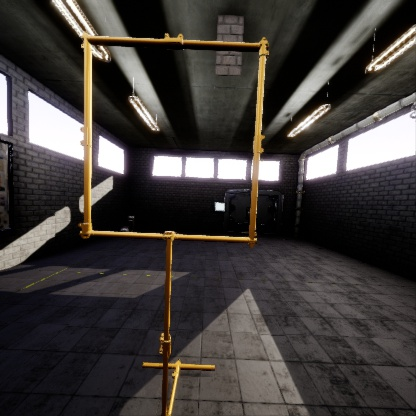
\includegraphics[width=\textwidth]{fig/sim}
	\end{minipage}
	\caption{Examples of samples with more background. On the left a sample augmented with an image from the Pascal VOC 2012 dataset. On the right a sample generated in the \textit{Daylight} Environment. Although on the left the background contains realistic data the scene does not align with the objects. Also the shadows to not fall correctly. With the simulated environment the general scene looks more realistic although the background is synthetic.}
	\label{fig:sim_vs_voc}
\end{figure}

\subsection{Training Set}

Four datasets are generated with 20 000 samples each. Dataset I contains samples generated by placing \ac{CAD}-models on uniformly coloured backgrounds; Dataset II contains samples generated by placing \ac{CAD}-models on backgrounds taken from the Pascal VOC dataset, Dataset III contains samples from the \textit{Dark} environment, Dataset III contains samples from all virtual environments. A fourth model is trained on a combination of Dataset II and IV (equal proportion).

Within the environment the camera is placed at random locations following these distributions:

\begin{equation}
x = \mathcal{U}(-30,30),\quad y = \mathcal{U}(-20,20),\quad z = \mathcal{N}(-4.5,0.5)),\quad
\phi = \mathcal{U}(0,0.1\pi),\quad \theta = \mathcal{U}(0,0.1\pi),\quad \psi = \mathcal{N}(-\pi,\pi)
\label{eq:distroexp}
\end{equation}

Where $ \mathcal{U}(a,b)$ is a uniform distribution between $a,b$ and $\mathcal{N}(\mu,\sigma^2)$ is a Gaussian distribution with mean $\mu$ and variance $\sigma^2$.

The models are tested on the real datasets described in \Cref{sec:datasets} as well as the simulated flight described in \Cref{sec:datagen:method}.


\subsection{Results}



\Cref{fig:context} display the results. It can be seen how using uniformly coloured backgrounds achieve almost no detection. Only on the simulated data a few objects could be detected.

In contrast using fully synthesized data achieves the best performance on the simulated data for low and high quality detections. It can be seen that almost all detections have an \ac{IoU} of more than 60\% and are thus good quality. On the real data the performance in low quality detections is comparable to the performance on the simulated data. However, in hiqh quality detections the performance drops significantly to an equal level of using real backgrounds.

Using real backgrounds performs poorer than using a fully synthesized environment in almost every case. However, for higher quality detections the performance is competitive to using a fully synthesized environment. Combining both methods does achieve at most the performance of using fully synthesized data. However, in most cases the performance is worse.   

\if false
\begin{table}[htbp]
	\caption{Results of different ways to generate context.}
	\begin{tabular}{lrrrrrr}
		\hline
		Name &  Sim Data0.4 &  Sim Data0.6 &  Sim Data0.8 &  Real Data0.4 &  Real Data0.6 &  Real Data0.8 \\
		\hline
		Real Backgrounds &         0.26 &         0.15 &         0.02 &          0.14 &          0.09 &          0.01 \\
		Uniform Backgrounds &         0.04 &         0.02 &         0.00 &          0.00 &          0.00 &          0.00 \\
		Various Environments &         0.32 &         0.31 &         0.08 &          0.33 &          0.10 &          0.01 \\
		Real + Various &         0.32 &         0.18 &         0.04 &          0.12 &          0.10 &          0.01 \\
		\hline
	\end{tabular}
	\label{tab:context}
\end{table}
\fi
\begin{figure}[htbp]
	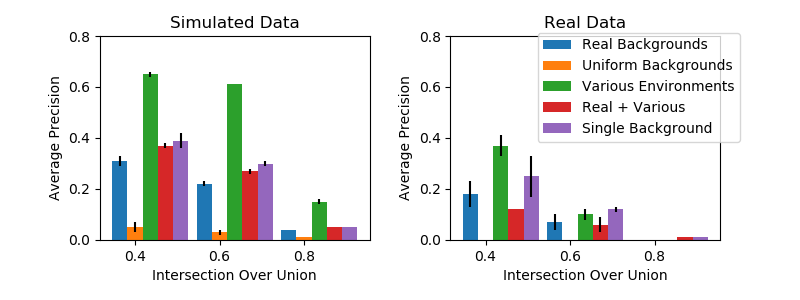
\includegraphics[width=\textwidth]{fig/context_bar}
	\caption{Results of different ways to generate context. Synthesizing more parts of the environment improves performance on both test sets. However, this only holds for weakly localized predictions.}
	\label{fig:context}
\end{figure}

\subsection{Discussion}

The results meet our hypothesis that using only uniformly coloured backgrounds is not enough to train an Object Detector for \ac{EWFO}. Providing more variance in the background is crucial to improve performance.

Despite having not seen a single real background, the model trained on fully synthesized data achieves the best performance on the real data. Even a model trained in a single virtual environment achieves competitive performance. Hence, it seems that synthesizing correct geometric/physical properties is more important than providing a large variance in background. However, the margin gets small for higher quality detections. Thus, the simulation of geometric/physical properties does not help for good localization.

\subsection{Conclusion}

We investigated the role context plays for the detection of \acp{EWFO} on \acp{MAV}. We can conclude that providing some background is crucial for the detection. Otherwise the detector performs poorly in simulation as well as the real world. Furthermore, synthesizing the whole environment benefits the detection on real images. However, most of the additional detections have not very accurate bounding boxes.

\section{Transferring the detector to an \ac{MAV} race}

Until now the conducted experiments where limited to relatively simple environments. In a real world application such as an \acp{MAV} race, much more objects are in sight. These can not only appear frontally but also in more difficult view angle. Furthermore, the objects can appear behind each other, such that in the empty part, another object is visible. This section studies whether the results obtained so far also apply in a more challenging environment. Therefore different architectures and training methods are evaluated on the synthetic test set described in \Cref{sec:datasets}.

Due to the challenges in this dataset we hypothesize that the detector trained so far will perform poorly on this dataset. In order to be able to handle overlapping objects in difficult angles, such situations should be included in the training set. In order to obtain such views different methods are compared.

A straightforward way is placing the camera randomly (within some margin) in order to cover a large variation of views on the object. That way the network can learn a general object representation and hopefully detect unseen objects from different view points. However, random  placement might not resemble the real world sufficiently. An \ac{MAV} does not appear at random places within a scene, especially not when it follows a racing track. We examine this by simulating a flight through a race court using AirSim's \ac{MAV} model and analyzing the relative object poses. We compare these to the relative poses obtained when placing the camera randomly using the distributions from \Cref{eq:distroexp}.

\begin{figure}
	\begin{minipage}{\textwidth}
		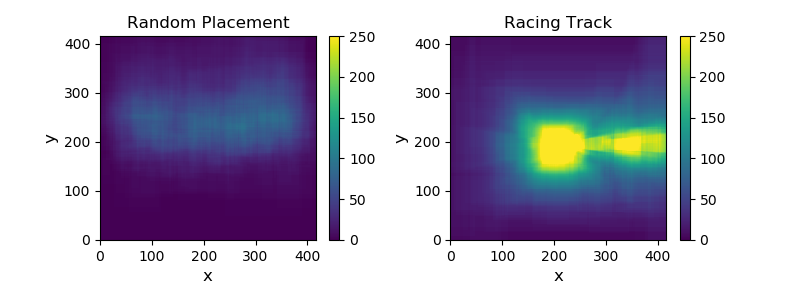
\includegraphics[width=\textwidth]{fig/heatmap_camplace}
		\caption{Object appearances when generating samples with random poses (left) and during a \ac{MAV} flight. During the flight the object appears mostly centered on the horizontal line.}
		\label{fig:heatmap_camplace}
	\end{minipage}
	\begin{minipage}{\textwidth}
		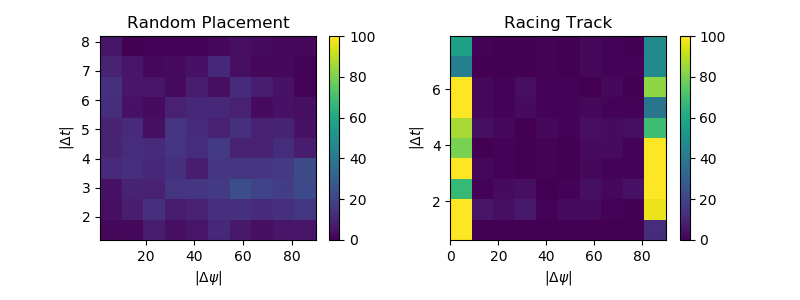
\includegraphics[width=\textwidth]{fig/hist2d_camplace}
		\caption{Histogram of object occurrences in yaw angle and distance relative to the camera. The random placement does rarely cover facing the object closely and frontally. }
		\label{fig:hist2d_camplace}
	\end{minipage}
\end{figure}

\Cref{fig:heatmap_camplace} shows the distribution of bounding boxes when created with random camera placement and when following a racing track. It can be seen how, when following the race track most of the objects are centered and distributed across the horizon, as camera focuses the next object frontally most of the time. In contrast, random placement leads to more evenly distributed object locations. This can also be seen in \Cref{fig:hist2d_camplace} where a 2D histogram of the yaw angle and distance with respect to the camera is displayed. Thereby 0 corresponds to facing the object frontally, 180 degrees facing the object from the back. It is apparent how the random placement covers a much larger range of relative angles, while in the racing track certain angles do not appear at all. Even more importantly the largest bins of the racing track is an angle of 0 and a distance between 0m and 4m. These bins are almost not present when placing the camera randomly. This is because close to the camera the field of view is small, while the area of the object faced frontally is big. Hence, the probability of an object ending up at this specific location is relatively low. Furthermore, when placing the camera randomly there are no samples further away than 8m. This is because in the race track the camera traverses the room from one end - where it can see almost all gates - to another. The probability that the randomly placed camera ends up in a similar position is relatively low.

The filters of \acp{CNN} are translation invariant by design but cannot inherently handle variation in rotation and scale. We hypothesize that the generation of samples with only one of the two methods can miss important object appearances. Random placement does not cover appearances that are typical for a autonomous drone race. On the other hand, only training on racing tracks might lead to a bias towards the created courses.

\subsection{Training Set}

\subsection{Results}
\subsection{Discussion}
\subsection{Conclusion}

\section{Transferring the detector to the real world}


In literature \cite{Krizhevsky2012a,Howard2013,Redmon,Liu} the application of image augmentation is a common tool to improve the detection performance. The experiments in \cite{Carlson2018} show how the incorporation of sensor effects particularly improves the performance of models learned on fully synthesized data. In the \ac{MAV} domain sensor and lens effects have a significant influence on the obtained sample. Hence, we hypothesize that the incorporation of these effects will improve the performance of the trained models. A total of  five image augmentation techniques are investigated.

\subsection{Results}

\begin{figure}[htbp]
	\centering
	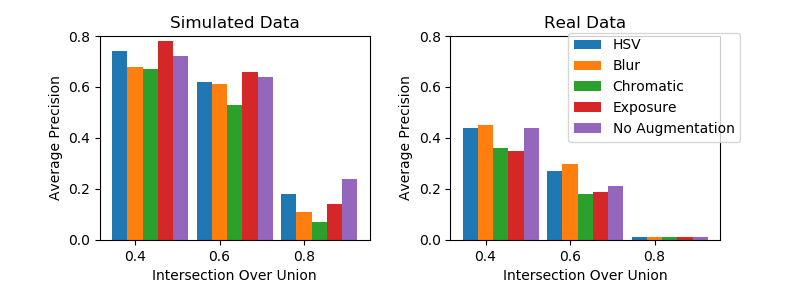
\includegraphics[width=\textwidth]{fig/pp_bar}
	\caption{Performance in terms of Average Precision for different methods  of image augmentation.}
	\label{fig:pp_bar}
\end{figure}

\Cref{fig:pp_bar} shows the results in terms of average precision in the training domain. On the simulated data variations in exposure improve the performance of low quality predictions slightly compared to using no augmentation. However, using no data augmentation achieves the best performance for high quality detections. The other effects have only minor influence. 

On the real data variations in HSV space as well as blurring improves the results compared to not using data augmentation. Incorporating chromatic aberration and variations in exposure lead to a deterioration in performance.

\subsection{Discussion}

In simulation the data augmentation has only a minor effect on low quality predictions, while the performance in high quality predictions decreases. As most effects are not really present in the test set this confirms that the models can learn a robust representation. Despite having more noise in the training data, the performance on the test set stays the same. However, the added noise leads to a lower quality in the predicted bounding boxes.

On the real data there is a stronger effect measurable. Variation in HSV and image blurring increase the performance compare to not using data augmentation. This meets our hypothesis that variations in HSV help to achieve a model that is more robust against changes in colour. Blur is one effect that can clearly be seen in the real world test set. Including this effect in the training process helped the model to perform better in the real world. Chromatic Aberration led to a significant improvement in \cite{Carlson2018} however, we cannot confirm these results. It is possible that our camera suffers only little from  chromatic aberration and thus including the effect in the training does not further help the prediction. The same holds for variations in exposure. 

\subsection{Conclusion}

We investigated whether including sensor effects present in the target domain in the data generation process can improve the detection. Therefore we modelled several effects that were observed when working with the camera or that improved the detection in experiments conducted in literature. Finally, image blurring improved the detection. Other effects led to a deterioration in performance.

We also investigated image augmentation by adding variations in HSV-space to evaluated whether this improves the robustness of the model, improving the performance on the real world dataset. We can confirm this hypothesis and conclude that this image augmentation should be part of the training process.


\section{Deploying the detector on a \ac{MAV}}

In the application of the detection of \acp{EWFO} on a \acp{MAV} detection accuracy is only one important metric. Equally relevant are inference speed and energy requirements. The example control loop in which the detector of this work is integrated, contains a filtering stage which fuses measurements of different sensors over time to infer a global state. This stage can deal with outliers and henceforth it can be more important ot have more bad detections in high frequency than only slow but good ones. This section studies the deployment of a detector for \acp{EWFO} on a \ac{MAV} in the example of the target system of this work. Therefore the performance-accuracy trade-off is studied and an experiment in a real world flight is conducted.

As explained in \Cref{sec:background} the execution time strongly depends on the used hardware as well as its low level implementation. Therefore the inference time of several layers is measured on the JeVois using the \textit{Darknet} framework. The results are displayed in \Cref{fig:bottleneck_jevois}. Each sample corresponds to the number of computations and their computational time in one layer. Dashed lines connect samples at the same resolution. It is apparent how the same amount of computations at a spatial resolution of 20x15 is more than 4 times faster than at a resolution of 160x120. We assume this is because parallelism is better exploited at the lower scale.

\begin{figure}[hbtp]
	\centering
	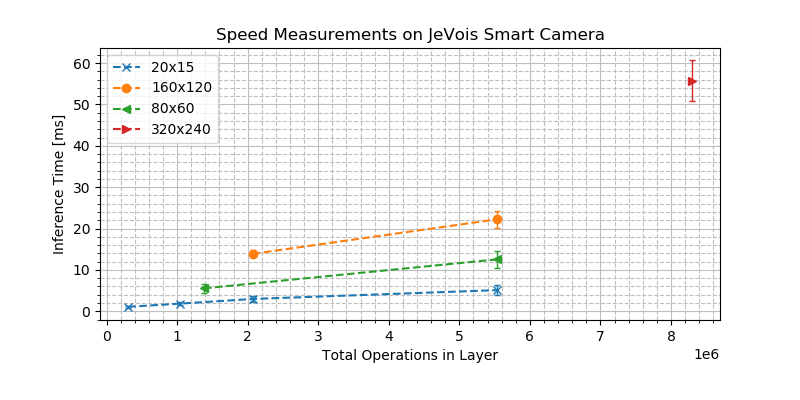
\includegraphics[width=0.8\textwidth]{fig/bottleneck_jevois}
	\caption{Inference Time of different layers on the JeVois. Each sample corresponds to the inference in a single layer. Dashed lines connect samples at the same resolution. It can be seen how an operation at a higher spatial resolution is significantly slower.}
	\label{fig:bottleneck_jevois}
\end{figure}


\textit{TinyYoloV3} is optimized to detect solid feature rich objects of multiple classes with a low computational budget. In order to sufficiently represent and distinguish such objects many weights are required. Hence, the network contains 9 layers and a final width of 1024. In contrast, the features of \acp{EWFO} are relatively simple hence less weights should be required. Therefore we hypothesize a thinner network should be able to learn the task equally well while being computationally more efficient.

The receptive field of \textit{TinyYoloV3} is 223 pixels which does not cover the full input image. For solid objects this is of minor impact as even if the network only sees an object part it can still learn to recognize it. However, this does not apply for \acp{EWFO} which are empty and do not contain any information in the object centre. Instead it can confuse an output layer that is assigned responsible to detect such an object. Therefore we hypothesize that more layers should improve the performance for larger objects. However, the c 

Yet, the complexity of large objects does not increase. Hence, we hypothesize that if the receptive field is large enough,  performance for larger objects. 

Another parameter are network width and depth.  The same condition holds for the number of layers. However, more layers also increase the receptive field. Hence, we expect the performance to increase as long as the receptive field does not fully capture the image.

In order to evaluate our hypothesis we perform an architecture evaluation by varying the number of layers filters and the receptive field. Before training the networks we tune the anchor box dimensions by performing a k-means clustering on t

Initially an architecture evaluation is performed. Therefore different architectures are trained and evaluated in terms of \ac{ap60}. As an architecture contains many parameters we can not simply vary each of them independently. Hence, three experiments are performed iteratively. We first describe them on a high level basis before explaining the exact changes. In a first step the width is decreased until a drop in performance is noticeable. In a second step the architecture with the lowest width but without performance drop is chosen and the depth is varied. Based on the results of this step we create a final model that combines the gained insights and tune the anchor boxes.

The scheme in which the architecture is changed is visualized in \Cref{fig:depth_changes}. The width of the baseline model is decreased stepwise by a factor of two. When decreasing depth only convolutional layers are removed while the pooling layers are kept such that the spatial resolution stays the same. When increasing depth 2 layers are inserted stepwise at the end of both branches. The results show how depth is mainly relevant to detect objects of larger scale. Hence, the final model consist of 5 common layers, 15 layers on the branch to detect larger objects and 2 layers on the branch to detect small objects.


This means most speed can be gained when reducing the number of computations in the early layers where the spatial resolution is high. In earlier experiments it could be seen that already a small amount of filters is enough to detect \acp{EWFO}. However, even evaluating 4 kernels at a resolution of 320x240 already takes 55 ms (\Cref{fig:bottleneck_jevois} red triangle). A total network of that size would require more than 200 ms and is thus too slow to be deployed in the control loop.

Current research mostly addresses to reduce the computations when the convolved volumes are deep or the operations are performed on \acp{CPU} that do not support floating point operations. However, the bottleneck on the JeVois happens at shallow volumes and the hardware can perform floating point operations. Furthermore, \acp{EWFO} consist of thin elements that are spread over large parts of the image. Hence, we hypothesize that simply reducing the image resolution will lead to large drops in performance. An alternative is to increase the stride parameter in the early layers of the network. This reduces the number of locations at which the kernel is evaluated. \acp{EWFO} are sparse and spread over large parts of the image, while most of the image does not contain useful information. Hence, we hypothesize that increasing the stride parameter in the early layers will perform better than reducing the image resolution.

\section{Experiments}

In order to answer this question we measure the inference time of different model architectures. This enables us to investigate the bottlenecks and thus optimize the model architecture. The JeVois Smart Camera uses an aspect ratio of 4:3. Therefore we change the network resolution accordingly. The JeVois Smart Camera has only limited memory available. Using a network architecture that goes beyond the memory simply results in a system crash. For example our baseline network runs performs one network evaluation in 700 ms. This is at a resolution of 160x120.

In order to evaluate our hypotheses the network is trained with different architectures. Subsequently, performance and inference time on the JeVois are measured.

The JeVois supports aspect ratios of 4:3 and resolutions of 160x120, 320x240 and 640x480. Although, \ac{FCN} do not depend on the image resolution, the object appearance can change at lower image resolution. Hence, during training the images are scaled to 160x160 or 320x320 respectively. The anchor boxes are scaled in similar fashion. Finally, as the input image resolution decreases, the output grid size decreases by the same factor. This is not desirable as the output resolution should stay the same. Hence, when decreasing the input image to 160x160 we remove the last pooling layer such that the output grid stays at 20,20 or 10,10 respectively.

\section{Results}

\begin{figure}[hbtp]
	\centering
	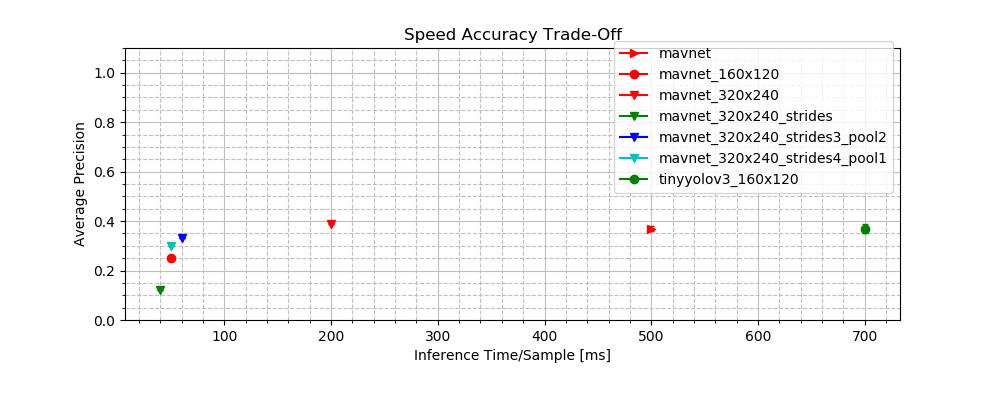
\includegraphics[width=0.8\textwidth]{fig/ap_speed_tradeoff}
	\caption{Inference Time of different layers on the JeVois. Each sample corresponds to a single layer. On the x-axis the total number of multiplications in that layer is displayed. It can be seen how an operation at a higher spatial resolution is significantly slower.}
	\label{fig:ap_speed_tradeoff}
\end{figure}

Due to their computational complexity deploying a \acp{CNN} on mobile devices is a challenging task


\Cref{fig:perf_width} shows the performance for thinner and wider networks. It is apparent how the performance only undergoes slight variations despite reducing the total number of weights by a factor 1000. \todo{retrain one in the middle to get variance, it should be more linear}


\begin{figure}[hbtp]
	\centering
	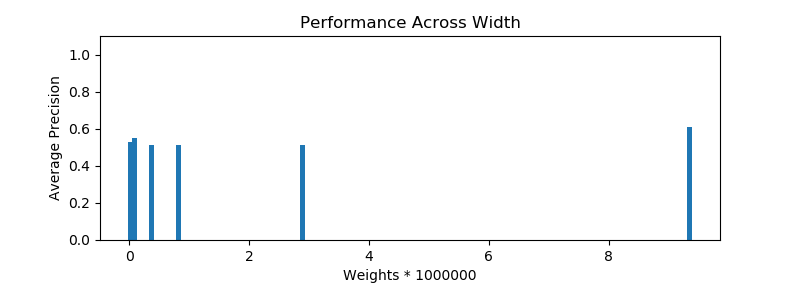
\includegraphics[width=\textwidth]{fig/perf_width}
	\caption{Performance in simulation when varying the amount of filters per layer. Starting from the baseline architecture with approximately 9 Mio. weights, the amount of filters per layer are decreased stepwise by a factor of 2. Only minor effects on performance can be seen, despite reducing the flexibility of the model.}
	\label{fig:perf_width}
\end{figure}

\begin{figure}[hbtp]
	\centering
	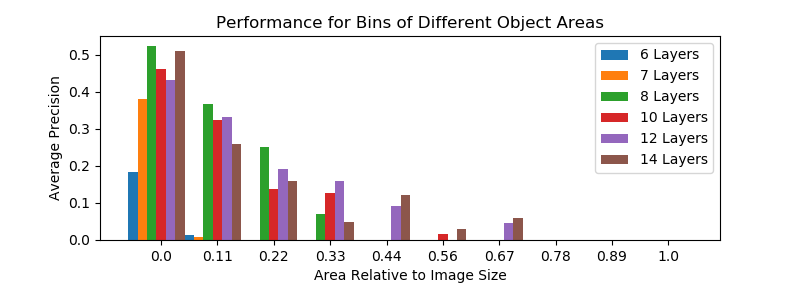
\includegraphics[width=\textwidth]{fig/depth_ap_size}
	\caption{Performance in simulation of models with varying depth and for bins of different size. It can be seen that the performance for larger objects increases with the amount of layers.}
	\label{fig:depth_ap_size}
\end{figure}

\Cref{fig:size_bins} shows the distribution of object sizes in the bins used for evaluation. It can be seen that most objects in the test set are further away. \todo{put some examples to show what each size actuall means}

\begin{figure}[hbtp]
	\centering
	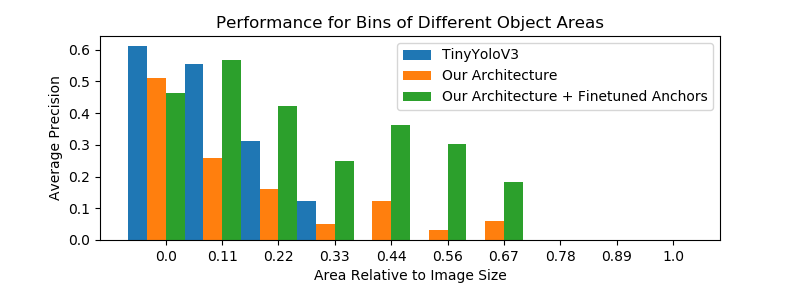
\includegraphics[width=0.8\textwidth]{fig/hyperparam_size}
	\caption{Architectural Changes when varying the depth. The upper graph shows in which order layers are removed. The lower graph shows how layers are added. Depth is increased by inserting two layers on each branch (green). }
	\label{fig:hyp}
\end{figure}

\begin{figure}[hbtp]
	\centering
	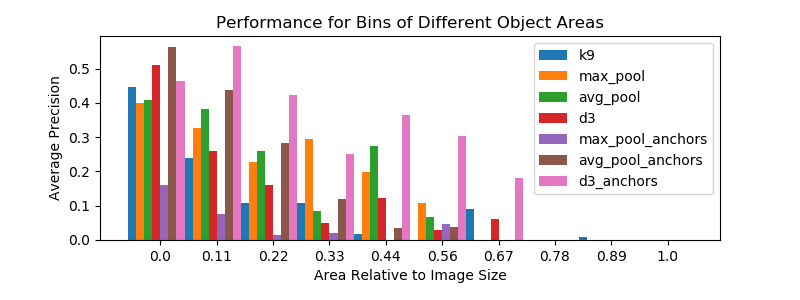
\includegraphics[width=\textwidth]{fig/rf_ap_size}
	\caption{Label distribution in bins of different object size. As the field of view is larger for objects further away, the proportion of small objects is higher.}
	\label{fig:size_bins}
\end{figure}

\subsection{Discussion}

The overall performance is only slightly affected when reducing the number of weights in terms of width and height. We can assume that this is because the objects we investigate are of quite simple structure. Intuitively the features to be considered are color, lines and edges in certain combinations. Hence, it seems logical that only a few filters are necessary to represent these shapes.

The performance in terms of different object sizes varies significantly for models with varying depth. Only deeper networks are able to detect larger objects. However, the complexity of the object does not increase for closer objects. In contrary the closer the objects are, the less context is visible. A very close object consists "only" of an orange square. Hence, it is unlikely that increased flexibility is the reason for the increase in performance. 

Instead it is more likely that the increased receptive field is the reason for the improved performance. In fact only the network with 14 layers has a receptive field of 414 an thus covers the whole image. Yet even this network cannot detect the largest objects. Thus the receptive field can not be the only reason for the lower performance on larger objects.

The current structure combines features distributed across space in a pyramid fashion. So 3-by-3 convolutions are performed layer by layer such until the whole image is covered. For \acp{EWFO} many of these steps are unnecessary as the objects are empty and the network should learn to ignore the empty part in the centre. It is possible that this structure gets confused by the parts that are present in the image centre.

\subsection{Conclusion}

We investigated how width affects the performance for the detection of \acp{EWFO}. We hypothesized that due to the low variance in the investigated object and the simple features, less filters are required than in the baseline architecture. We can confirm this hypothesis as we see that the width can be decreased by a factor of 10 without loosing performance. This leads to a reduction of weights by a factor of 1000. 

Furthermore, we investigated how depth affects the performance of the model. We hypothesized that a shallow network should be able to detect the object as it only consists of relatively simple features. We can see how depth is required in order to cover the whole input image. Hence, we cannot fully conclude whether depth is required for the increased flexibility or simply due to the receptive field. 





